\begin{figure}
\centering
    \begin{subfigure}{.45\textwidth}
        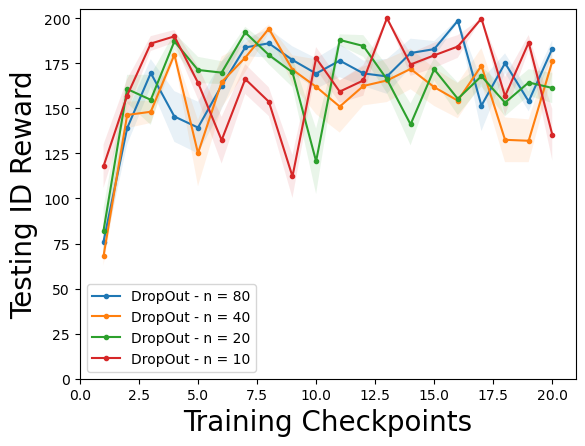
\includegraphics[width=\textwidth]{sections/011_icml2022/resources/CartPole-v0-mean_reward_-testing-hyperparameter-n_sample-dropout.png}  
    \end{subfigure}
        \begin{subfigure}{.45\textwidth}
        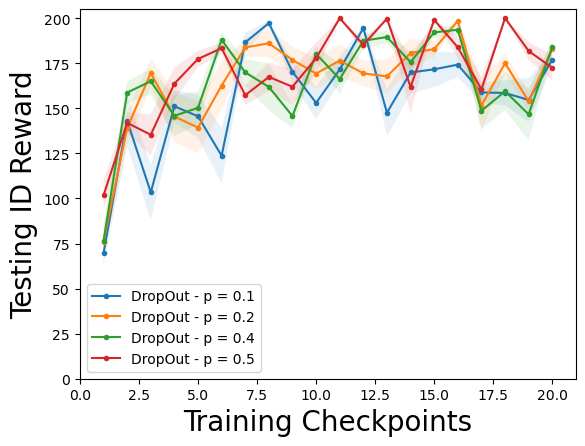
\includegraphics[width=\textwidth]{sections/011_icml2022/resources/CartPole-v0-mean_reward_-testing-hyperparameter-p-dropout.png}  
    \end{subfigure}
    
    \begin{subfigure}{.45\textwidth}
        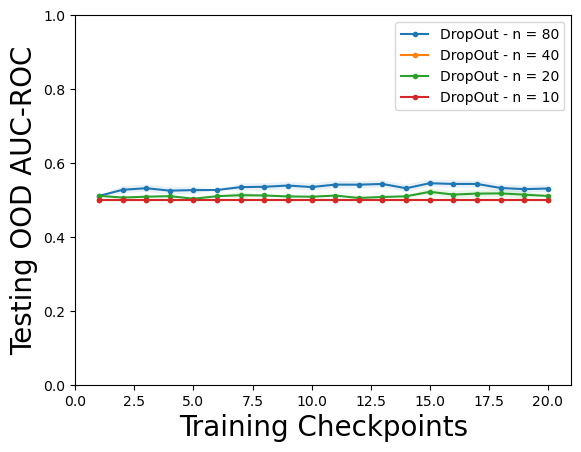
\includegraphics[width=\textwidth]{sections/011_icml2022/resources/CartPoleOOD-v0-AUC-ROC-epistemic_-testing-hyperparameter-n_sample-dropout.png}
    \end{subfigure}
        \begin{subfigure}{.45\textwidth}
        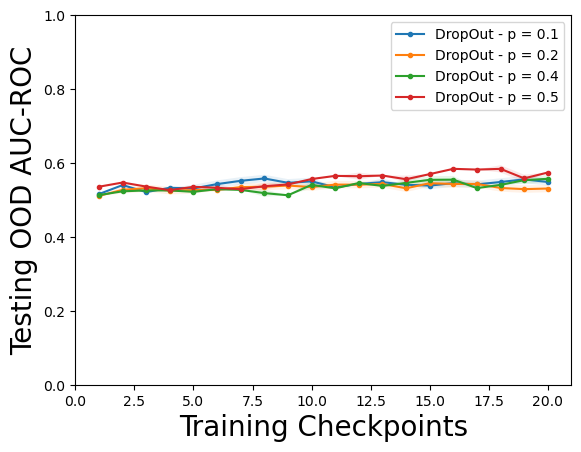
\includegraphics[width=\textwidth]{sections/011_icml2022/resources/CartPoleOOD-v0-AUC-ROC-epistemic_-testing-hyperparameter-p-dropout.png}
    \end{subfigure}
        \vspace{-3mm}
    \caption{Hyper-parameter study for DropOut w.r.t. the number of samples $n$ and the dropout probability $p$. Ideally, an uncertainty aware-model should achieve high reward and high OOD detection scores.}
    \label{fig:hyperparameter-dropout-cartpole}
    \vspace{-4mm}
\end{figure}